\subsubsection*{Water movement within the roots} \label{sssec:xylem}

Since water movement within the roots is often needed, it is implemented directly in CPlantBox (in the class XylemFlux) following \cite{meunier2017hybrid}. However, usage is optional, and any other transport code can be used (e.g. if solutes are considered). XylemFlux sets up the linear system, and the sparse linear system is then solved in Python using scipy (using the class XylemFluxPython defined in xylem$\_$flux.py).

The following example is based on benchmark M3.1 \citep{schnepf2019call} with constant conductivities, but not with a given root system, but a simulated one.

\lstinputlisting[firstline=1, language=Python, caption=Example 6b]{examples/example6b_xylemflux.py}
\begin{itemize}

\item[11-15] All parameters that will be used later on.

\item[18-23] The root system (similar to last section). 

\item[26-31] The MappedRootSystem is wrapped with the XylemFluxPython class, which extends the XylemFlux class, which computes the xylem matric flux potential. L27, L28 sets the radial and axial conductivity. L29 retrieves the root system nodes for later visualisation. The pressure surrounding the the root system is either defined as pressure surrounding each root segment, or as soil cells, in which the root segments are located. L30, L31 sets a soil containing of one single cell with index 0. 

\item[34-36] XylemFluxPython defines solvers like solve$\_$dirichlet for Dirichlet boundary condition (predefined collar matric potential), solve$\_$neumann for Neumann boundary condition (predefined collar flux), and solve which switches between Dirichlet and Neumann at some critical pressure (the plant wilting point).
The arguments of solve$\_$dirichlet are the simulation time (to calculate age dependent conductivities), the root collar pressure head, the pressure around the root collar, the soil matric potential around the root segments or per soil cell, and a boolean value that decides if the potentials are given per soil cell (True) or per segments (False). The return value $rx$ contains the xylem matric potentials per segment. L35 calculates the fluxes into the soil (negative values mean into the root). The bool argument determines if we approximate the flux, or use the exact solution by \cite{meunier2017hybrid}.
L36 determines the root collar flux.

\item[39-43] Plots the results.

\item[46-49] Creates the VTK plot, adding the soil matric potentials and fluxes. L49 picks either $rx$ or $fluxes$ for vizualisation, see Figure \ref{fig:xylemfluxa} and \ref{fig:xylemfluxb}.

\end{itemize}

It is possible to set conductivties per root type (see XylemFlux::setKr, and setKx), and root age dependent conductivities per root type using linear lookup tables (see XylemFlux::setKrTables, and setKxTables).

\begin{figure}
\begin{subfigure}[c]{0.5\textwidth}
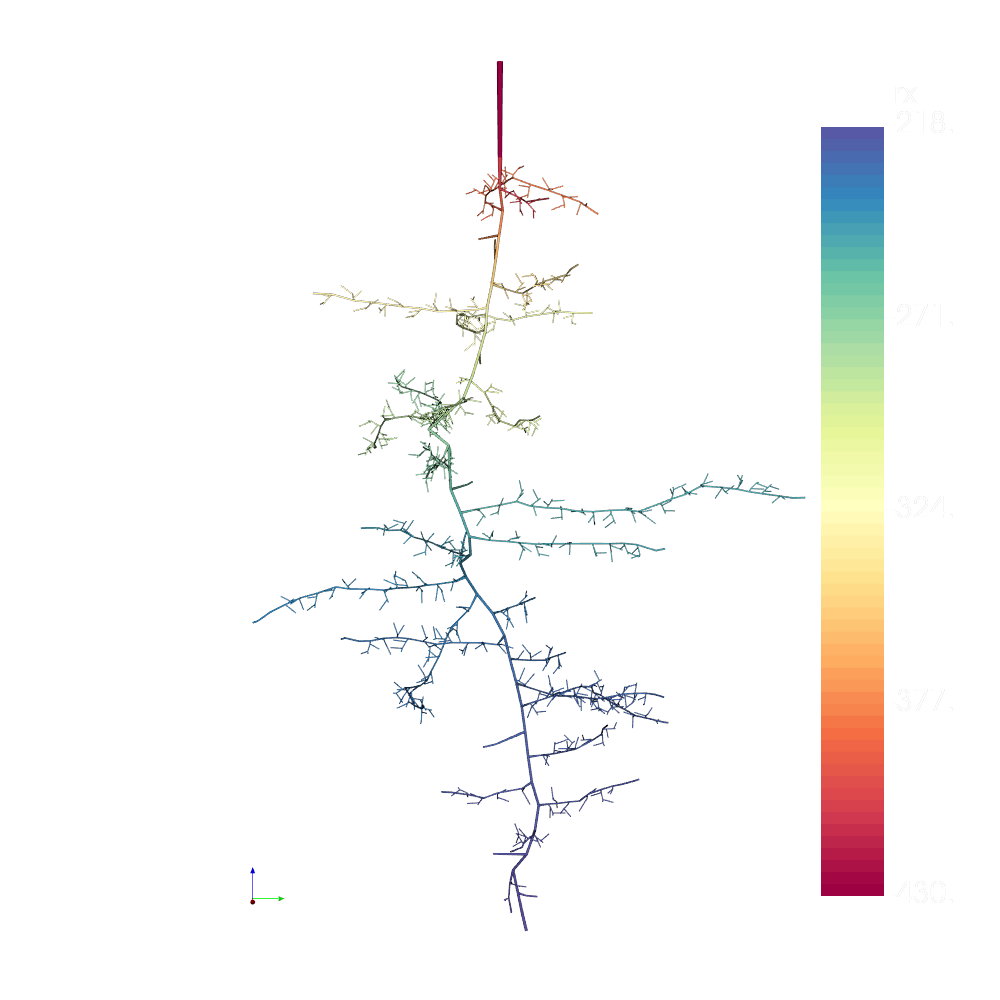
\includegraphics[width=0.99\textwidth]{example6b.png}
\subcaption{Anagallis} \label{fig:xylemfluxa}
\end{subfigure}
\begin{subfigure}[c]{0.5\textwidth}
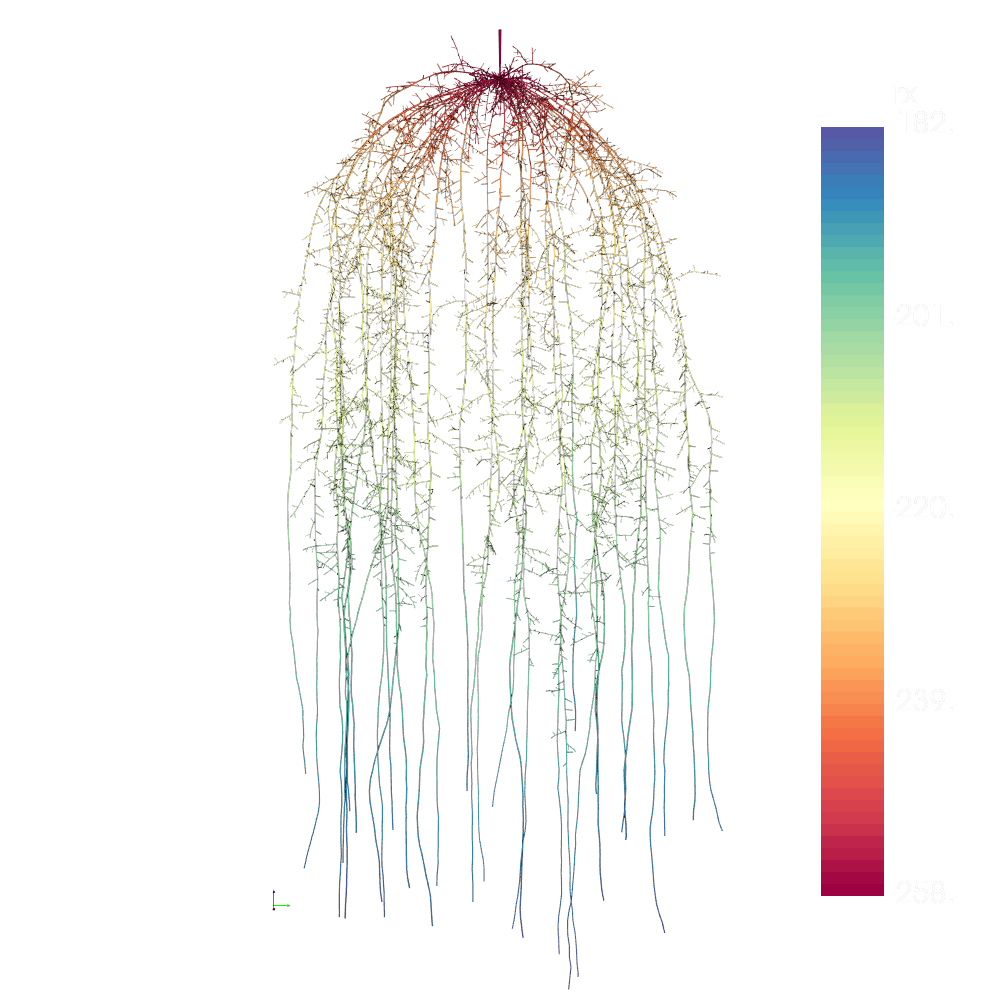
\includegraphics[width=0.99\textwidth]{example6b_2.png}
\subcaption{Maize} \label{fig:xylemfluxb}
\end{subfigure}
\caption{Calculated xylem matric potential (cm)} 
\end{figure}

\subsection{Stomatal modul} \label{ssec:stomatal}

The following example presents the stomatal modul (see file example6e$\_$xylemflux$\_$variable$\_$gs.py). The actual evapotranspiration (ETa) of the plant is determined according to environmental parameters, root and leaf surface, and maximal stomatal conductance (gmax). 
%\lstinputlisting[firstline=1, language=Python, caption=Example 6e]{../examples/example6e_xylemflux_variable_gs.py}
\begin{itemize}

\item[11-19] Part of the parameters that will be used later on.

\item[18-23] The root system (similar to last section). 

\item[21-25] Creation of the plant object, definition of the grid and simulation of the plant growth.

\item[38-42] Set the parameters for the calculation of the actual leaves radial conductivity (gs) and ETa using the equations of [TOADD].

\item[44-48] Get the plant nodes and tips to set the Neumann boundary conditions (i.e. 0 axial flux is set at the plant nod tips (i.e: water only enters/leaves the plant by radial flux)

\item[51] Solve the water flux using the Neumann boundary conditions. The program then loops on the calculation of ETa, xylem potential, and gs until convergence or after having done 1000 loops. p$\_$linit and gmax are respectively the initial leaf xylem potential and initial leaf radial conductivity used in the loop.

\item[52] Calculation of the radial fluxes of each plant segment.

\item[53] Gives an overview of the water fluxes in the plant. If show$\_$matrices = True, the matrices with the axial and radial water fluxes for each plant segment is shown.

\item[62-72] Plots the results (see Figure \ref{fig:stomata} and \ref{fig:stomatb}).

\item[75-78] Creates the VTP file, which can then be opened in Paraview.

\end{itemize}

\begin{figure}
\begin{subfigure}[c]{0.5\textwidth}
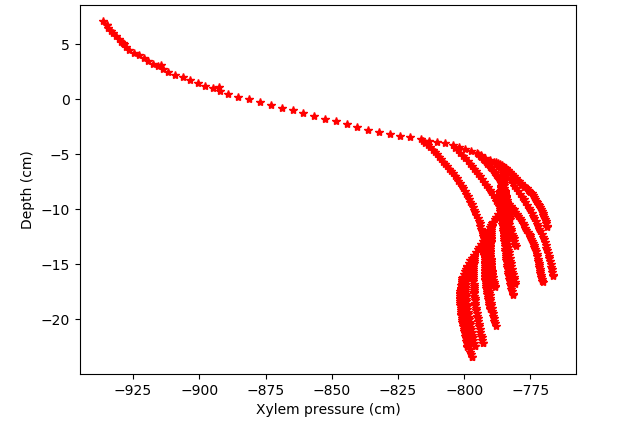
\includegraphics[width=0.99\textwidth]{example6e.png}
\subcaption{Calculated xylem matric potential (cm)} \label{fig:stomata}
\end{subfigure}
\begin{subfigure}[c]{0.5\textwidth}
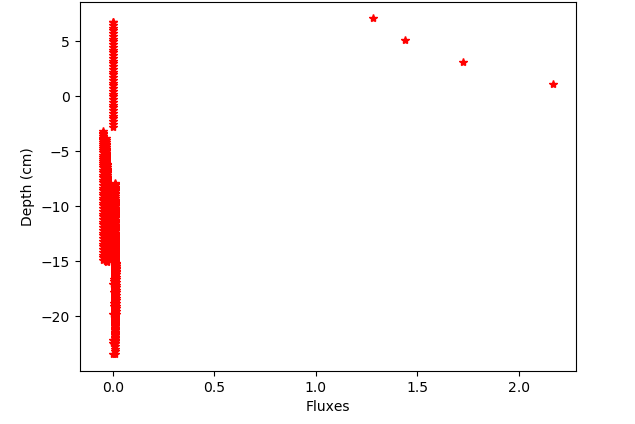
\includegraphics[width=0.99\textwidth]{example6e_2.png}
\subcaption{Radial water fluxes} \label{fig:stomatb}
\end{subfigure}
\caption{xylem potential and radial water fluxes per segment} 
\end{figure}


